\section{Experiments}
\label{sec:evaluation}

This section should substantiate the paper's main claims.
Start by naming the evaluation tasks, datasets, metrics, and baselines.

\begin{figure*}[!h]
  \centering
  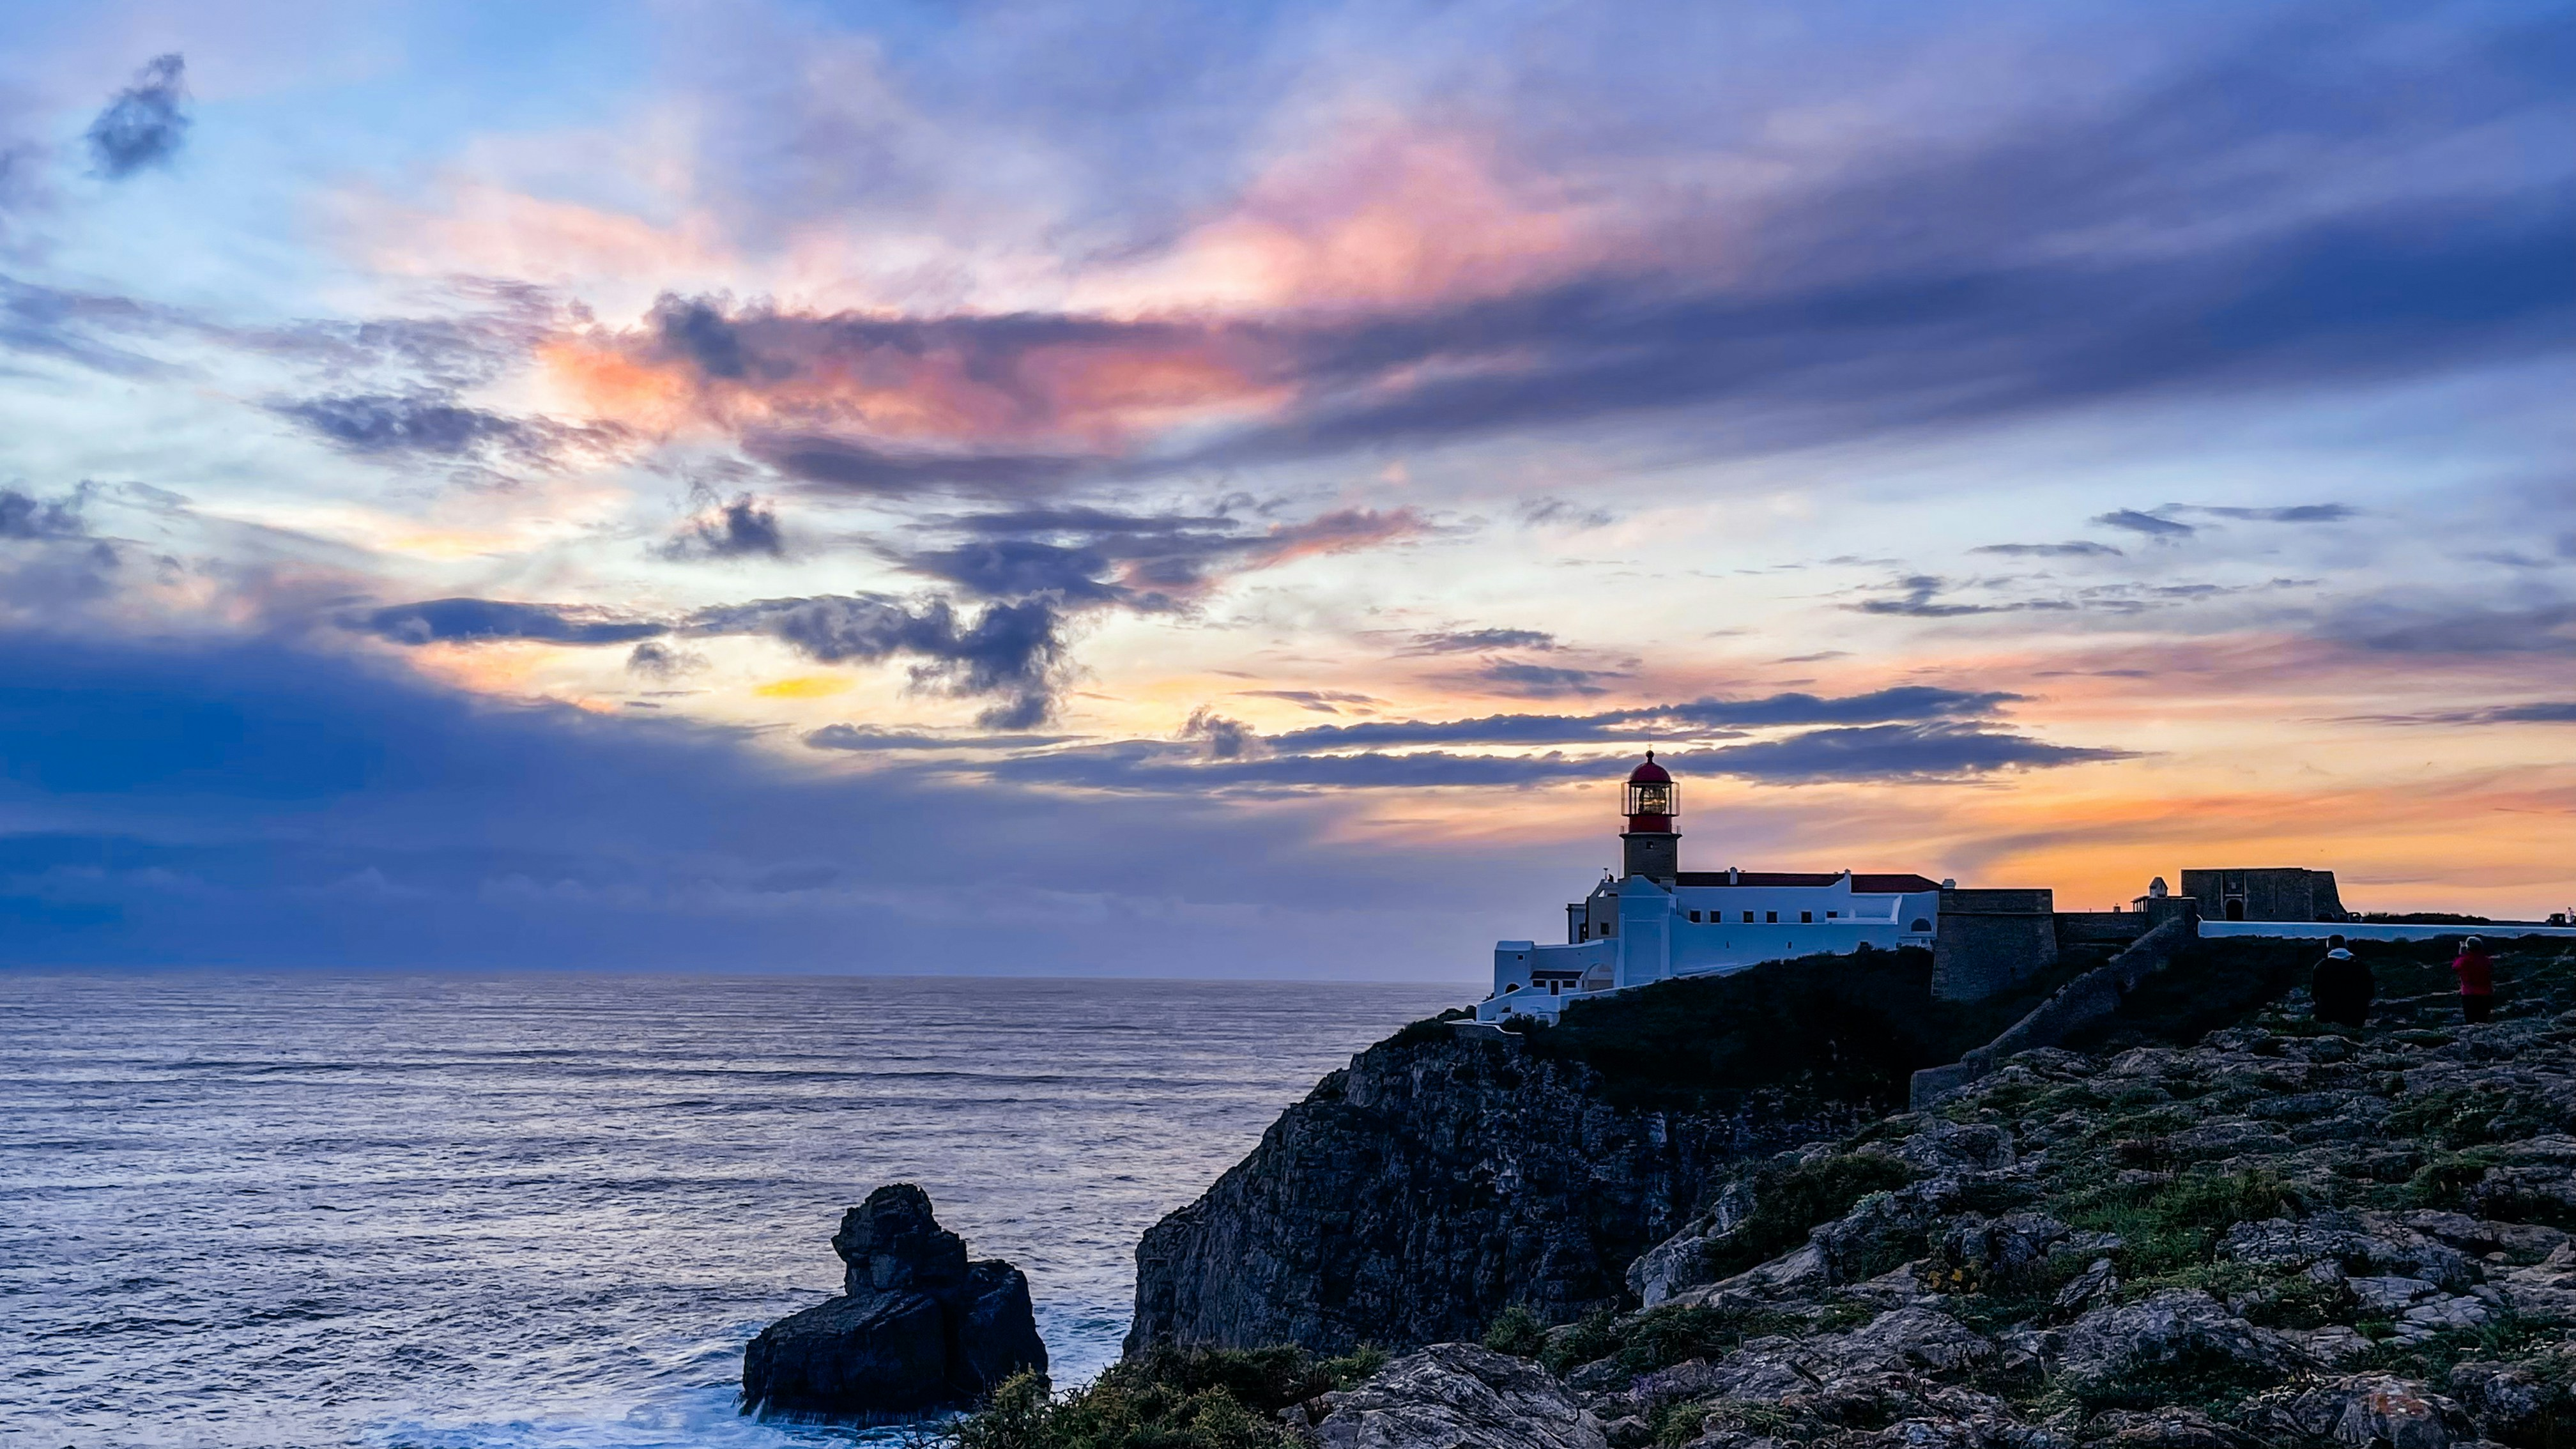
\includegraphics[width=0.9\linewidth]{pngs/image3.png}
  \caption{\textbf{Qualitative comparison.} Replace this placeholder with representative outputs, examples, or visual comparisons.}
  \label{fig:qualitative_results}
\end{figure*}

\subsection{Experimental Setup}

Describe the benchmark protocol, baselines, metrics, and statistical testing procedure.
Make clear which results are produced by the proposed method and which are reproduced from prior work.

\subsection{Main Results}

Present the primary quantitative results.
Use tables for numeric comparisons and figures for trends or qualitative behavior.
Discuss the result in terms of the claims made in the introduction.

\subsection{Ablation Study}

Isolate important design choices and report their effect.
Each ablation should answer a specific question about the method.

\subsection{Limitations}

Describe known limitations, failure cases, and conditions under which the method should not be used.
This improves the usefulness and credibility of the final paper.
